\chapter{Le primitive di base}

{ }\hfill\textbf{Livello:} principiante\\ \\
\noindent

Per spostare la tartaruga nell'area di disegno si usano comandi predefiniti chiamati ``primitive''. In questo capito scopriremo le primitive di base che permettono di pilotare la tartaruga nell'area di disegno.


\section{Le primitive indispensabili}
\begin{itemize}
	\item \texttt{Avanti o Av numero passi}\hspace {4cm } \textcolor{red}{ \texttt{Avanti 50}}\\
	Sposta la tartaruga in avanti di un certo numero di passi, nella direzione nella quale è disposta.
	
	\item \texttt{Indietro o In numero passi}\hspace {4cm } \textcolor{red}{ \texttt{In 100}}\\
	Sposta la tartaruga indietro di un certo numero di passi, nella direzione nella quale è disposta.

	\item \texttt{RuotaDestra o DX angolo}\hspace {4cm } \textcolor{red}{\texttt{DX 90}}\\
	Ruota la tartaruga a destra di un certo numero di gradi, in relazione alla direzione nella quale è disposta.

	\item \texttt{RuotaSinistra o SX angolo}\hspace {4cm } \textcolor{red}{\texttt{SX 90}}\\
	Ruota la tartaruga a sinistra di un certo numero di gradi, in relazione alla direzione nella quale è disposta.

	\item \texttt{PulisciSchermo o PS}\hspace {4cm } \textcolor{red}{ \texttt{PS}}\\
	Pulisce l'area di disegno.

	\item \texttt{MostraTartaruga o MT}\hspace {4cm } \textcolor{red}{ \texttt{MT}}\\
	Rende visibile la tartaruga.

	\item \texttt{NascondiTartaruga o NT}\hspace {4cm } \textcolor{red}{ \texttt{NT}}\\
	Rende invisibile la tartaruga (disegnare diventa più veloce).

	\item \texttt{PennaSù o PS}\hspace {4cm } \textcolor{red}{ \texttt{PS}}\\
	La tartaruga non lascia traccia quando si sposta.

	\item \texttt{PennaGiù o PG}\hspace {4cm } \textcolor{red}{ \texttt{PG}}\\
	La tartaruga lascia una traccia muovendosi (situazione predefinita).

	\item \texttt{Ripeti numero intero elenco}\hspace {4cm } \textcolor{red}{ \texttt{Ripeti 5[Avanti 50 DX 45]}}\\
	Ripete un elenco di istruzioni per un numero di volte.
\end{itemize}


\section{Cominciamo a disegnare}
In questa parte impareremo a disegnare un quadrato, un triangolo equilatero ed un qualsiasi altro poligono regolare\textellipsis. Un poligono regolare è una figura geometrica avente tutti i lati e tutti gli angoli congruenti fra loro (cioè uguali). La somma degli angoli interni è pari a $$(n-2) \times 180^{\circ}$$ dove $n$ è il numero dei lati del poligono regolare. La somma degli angoli esterni è sempre pari a $360^{\circ}$.

\subsection{Il quadrato}
\begin{center}
	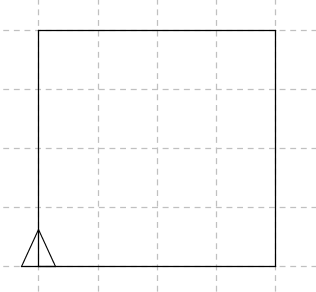
\includegraphics{pics/bases-carre.png}
\end{center}
\noindent Per disegnare questo quadrato di 200 passi di lato, occorre scrivere:
\lstinline!Av 200 DX 90 Av 200 DX 90 Av 200 DX 90 Av 200 DX 90!Possiamo notare che ripetiamo il disegno di ciascun lato per quattro volte, possiamo quindi sintetizzare il programma così: \lstinline!Ripeti 4[Av 200 DX 90]!.


\subsection{Il triangolo equilatero}
\begin{center}
	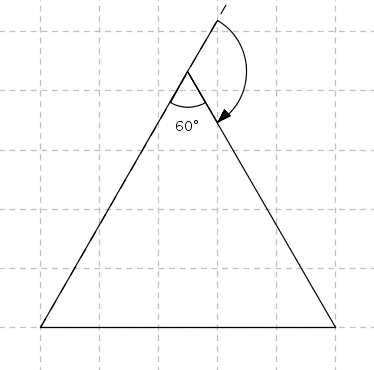
\includegraphics{pics/bases-triangle.png}
\end{center}
Adesso impariamo a disegnare questo triangolo equilatero di lato 150 passi.
Il programma avrà questa forma generica che abbiamo imparato a proposito del quadrato: \lstinline! Ripeti 3[Av 150 DX ....]!.
Dobbiamo determinare l'angolo di rotazione della tartaruga. In un triangolo equilatero i tre angoli interni sono uguali fra loro e quindi, visto che la somma degli angoli interni di un triangolo è $180^{\circ}$, ciascun angolo sarà pari a $\frac{180^{\circ}}{3}=60^{\circ}$. Ricordiamoci, guardando la figura, che l'angolo di rotazione della tartaruga è l'angolo esterno, non quello interno al triangolo. L'angolo di rotazione sarà quindi $180^{\circ}-60^{\circ}=120^{\circ}$. Il comando da fornire sarà quindi \lstinline!Ripeti 3[Av 150 DX 120]!.


\subsection{L'esagono}
\begin{center}
	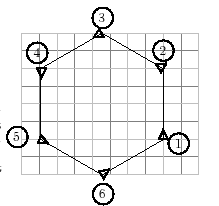
\includegraphics{pics/bases-hexagone.png}
\end{center}

\begin{lstlisting}
Ripeti 6[Av 80 DX ....]
\end{lstlisting}
Occorre determinare anche qui l'angolo di rotazione della tartaruga. Riflettiamo sul fatto che la tartaruga, una volta completato il disegno di tutti i lati, sarà tornata nella posizione di partenza e con la direzione originaria. Questo significa che avrà compiuto una rotazione totale di $360^{\circ}$, in sei passi (tanti quanti sono i lati). Quindi ad ogni passo avrà compiuto una rotazione pari a $\frac{360^{\circ}}{6}=60^{\circ}$. Il comando da fornire sarà quindi \lstinline!Ripeti 6[Av 80 DX 60]!.



\subsection{Un poligono regolare generico}
Nei fatti, il ragionamento che abbiamo applicato per disegnare l'esagono, è valido per qualsiasi poligono regolare, visto che la tartaruga dovrà ruotare di $360^{\circ}$ in passi successivi uguali fra loro. Se indichiamo con $n$ il numero dei lati la formula per calcolare l'angolo di rotazione da compiere per ciascun passo sarà pari a $\frac{360^{\circ}}{n}$. Per esempio
\begin{itemize}
	\item Per disegnare un triangolo equilatero di lato 100: \lstinline!Ripeti 3[Av 100 DX 120]    # (360:3=120)!.
	\item Per disegnare un pentagono regolare di lato 50: \lstinline!Ripeti 5[Av 50 DX 72]    # (360:5=72)!.
	\item Per disegnare un ennagono regolare di lato 20: \lstinline!Ripeti 9[Av 20 DX 40]    # (360:9=40)!.
	\item Per disegnare un \textellipsis 360-gono regolare di lato 2: \lstinline!Ripeti 360[Av 2 DX 1]    # (360:360=1)!. Questa figura è molto vicina ad una circonferenza!
	\item Per disegnare un ettagono di lato 120: \lstinline!Ripeti 7 [Av 120 DX 360/7]  # quanto fa?!.
\end{itemize}


\section{Definire una procedura}
Poiché non vogliamo riscrivere ogni volta le stesse istruzioni per disegnare un quadrato, un triangolo \textellipsis è meglio salvarle in ``procedure''. Per definire una procedura, apri l'editor. Una procedura comincia con la primitiva \texttt{Per} e termina con la primitiva \texttt{Fine}. Per esempio per inserire le istruzioni per disegnare il quadrato in una procedura:
\begin{lstlisting}
Per Quadrato
	Ripeti 4[Av 100 DX 90]
Fine
\end{lstlisting}
Quindi chiudiamo l'editor cliccando sul bottone che raffigura la tartaruga. La procedura verrà salvata. Ora scrivendo semplicemente \texttt{Quadrato} verrà disegnato un quadrato.


\section{Qualche esercizio}
Ciascun quadretto nelle figura ha lato pari a 10 punti. Prova a disegnare questa figura usando otto procedure:
\begin{itemize}
	\item Una procedura chiamata \texttt{Quadrato} che disegna il quadrato principale della casa.
	\item Una procedura chiamata \texttt{Triangolo} che disegna il tetto come un triangolo equilatero.
	\item Una procedura chiamata \texttt{Porta} che disegna una porta rettangolare.
	\item Una procedura chiamata \texttt{Camino} che disegna il camino.
	\item Una procedura chiamata \texttt{SpostaAB} che sposta la tartaruga dal punto A al punto B.
	\item Una procedura chiamata \texttt{SpostaBC} che sposta la tartaruga dal punto B al punto C (attento, devi alzare la penna della tartaruga).
	\item Una procedura chiamata \texttt{SpostaCD} che sposta la tartaruga dal punto C al punto D.
	\item Una procedura generale chiamata  \texttt{casa} che disegna l'intera casa utilizzando tutte le precedenti procedure.
\end{itemize}
\label{maison}
\begin{center}
	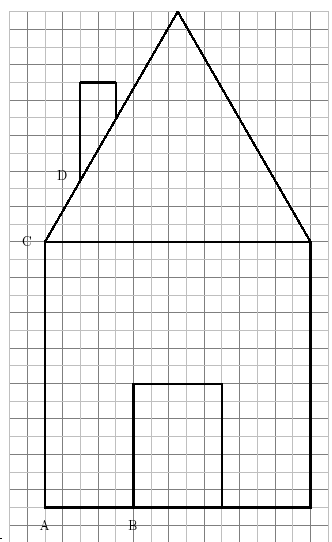
\includegraphics[scale=0.6]{pics/bases-maison.png}
\end{center}